% =====================================================================
%  MoodBloom — Final Pitch to the Industry Committee
%  Beamer deck · 7 sections · 24 slides (mapped 1:1 to the official outline)
%  Anchored to v1.6 (final-submission state) · HEAD 0e55021a
%  v1.6 is the v1.5 PATCH wave — still Sprint 5; the project is five sprints.
%  + Appendix A1–A8 (technical backup, separately numbered, not presented)
%  Dual-coded: technical proof for the commentators + a business
%  throughline (orange "Business:" lines) for the industry committee.
%  Every numeric/code claim traces to a real repo artifact — see the
%  companion speaker-script.md and qa-prep.md for evidence pointers.
%
%  COMPILE: Overleaf (pdfLaTeX) or `pdflatex presentation.tex` twice.
% =====================================================================
\documentclass[aspectratio=169,11pt]{beamer}

% ---- Theme : Madrid active for out-of-the-box compile. On Overleaf you
% ---- may swap to Metropolis (comment Madrid+colortheme, uncomment metropolis).
\usetheme{Madrid}
\usecolortheme{seahorse}
% \usetheme{metropolis}

\usepackage[utf8]{inputenc}
\usepackage[T1]{fontenc}
\usepackage{lmodern}
\usepackage{amsmath}
\usepackage{graphicx}
\usepackage{listings}
\usepackage{xcolor}
\usepackage{booktabs}
\usepackage{tikz}
\usetikzlibrary{arrows.meta,positioning,shapes.geometric}
\usepackage{hyperref}
\usepackage{tabularx}
\usepackage{pgfpages}

\IfFileExists{fontawesome5.sty}{\usepackage{fontawesome5}}{}
\providecommand{\faMicrochip}{}
\providecommand{\faProjectDiagram}{}
\providecommand{\faShieldAlt}{}
\providecommand{\faLeaf}{}
\providecommand{\faRobot}{}
\providecommand{\faLock}{}
\providecommand{\faChartLine}{}
\providecommand{\faCheckCircle}{}
\providecommand{\faExclamationTriangle}{}
\providecommand{\faChartPie}{}
\providecommand{\faBalanceScale}{}
\providecommand{\faCoins}{}

% ---- MoodBloom palette ----
\definecolor{moodgreen}{HTML}{2E7D5B}
\definecolor{moodgreendark}{HTML}{1F4E3D}
\definecolor{moodorange}{HTML}{E65100}
\definecolor{moodred}{HTML}{C62828}
\definecolor{moodyellow}{HTML}{F9A825}

\setbeamercolor{title}{fg=moodgreendark}
\setbeamercolor{frametitle}{bg=moodgreen,fg=white}
\setbeamercolor{structure}{fg=moodgreen}
\setbeamerfont{frametitle}{size=\large,series=\bfseries}

% Business throughline helper.
\newcommand{\biz}[1]{\vspace{0.3em}\par{\footnotesize\color{moodorange}\faChartPie\ \textbf{Business:} #1}}

% ---- Code listing styles (NB: `listings` has no "Dart" language). ----
\lstdefinestyle{dartstyle}{
  language=Java,
  morekeywords={final,enum,switch,throw,Future,await,async,expect,reason},
  basicstyle=\ttfamily\scriptsize,breaklines=true,frame=single,
  backgroundcolor=\color{gray!8},numbers=none,
  keywordstyle=\color{moodgreendark}\bfseries,
  commentstyle=\color{gray!70}\itshape,stringstyle=\color{moodorange}
}
\lstdefinestyle{rulestyle}{
  language=JavaScript,
  morekeywords={allow,update,if,request,resource,diff,affectedKeys,hasOnly},
  basicstyle=\ttfamily\scriptsize,breaklines=true,frame=single,
  backgroundcolor=\color{gray!8},numbers=none,
  keywordstyle=\color{moodgreendark}\bfseries,
  commentstyle=\color{gray!70}\itshape,stringstyle=\color{moodorange}
}
\lstset{style=dartstyle}

% ---- Speaker-notes mode (pick ONE) ----
\setbeameroption{hide notes}
% \setbeameroption{show notes}
% \setbeameroption{show notes on second screen=right}

\title{MoodBloom}
\subtitle{An Enterprise Mobile App, Engineered as a Five-Sprint Multi-Agent AI Orchestration}
\author[Group 2]{Group 2 \\ \small Kraiwich Jaiton \and Teerin Kittichaicharoen \and Theerawat Patthawee \and Jedsarit Fanpimiy \and Napat Chang-ekwong}
\institute{KMUTT \textperiodcentered\ CSC231 + CSC234 \textperiodcentered\ Semester 2/2568}
\date{Final Presentation \textperiodcentered\ \texttt{v1.6 \textperiodcentered\ 0e55021a} \textperiodcentered\ \today}

% =====================================================================
\begin{document}

% =====================  SECTION 1 — TITLE & TEAM  ====================

% ---- Slide 1 : Title ----
\begin{frame}[plain]
  \centering
  \vfill
  {\Huge\bfseries\color{moodgreendark} MoodBloom}\\[0.3em]
  {\color{moodgreen}\rule{0.45\textwidth}{1.2pt}}\\[0.8em]
  \begin{minipage}{0.82\textwidth}\centering
    \normalsize\itshape
    A compassionate cross-platform mood-tracker that turns daily
    emotional logging into the slow cultivation of a personal garden ---
    engineered as a five-sprint multi-agent AI orchestration.
  \end{minipage}\\[1.2em]
  {\small Group 2 \textperiodcentered\ KMUTT \textperiodcentered\ CSC231 Agile SE + CSC234 User-Centric Mobile Dev \textperiodcentered\ Semester 2/2568}\\[0.5em]
  {\footnotesize\ttfamily release v1.6 (Sprint 5 patch) \textperiodcentered\ commit 0e55021a \textperiodcentered\ \today}
  \vfill
  \note{Orchestrator (Theerawat). Warm opener, value prop verbatim, name the three lenses: business opportunity, therapeutic safety, engineering maturity. speaker-script.md, Slide 1.}
\end{frame}

% ---- Slide 2 : Team ----
\begin{frame}{The Team --- in Three Orchestration Roles}
\begin{columns}[T,onlytextwidth]
  \begin{column}{0.32\textwidth}
    \textbf{\color{moodgreen}\faMicrochip\ Orchestrator}\\[0.3em]
    Plans sprints, dispatches subagents, owns Plan Mode + approval gates.\\[0.6em]
    \small Theerawat Patthawee \textit{(Lead)}
  \end{column}
  \begin{column}{0.32\textwidth}
    \textbf{\color{moodorange}\faProjectDiagram\ Architect / Reviewer}\\[0.3em]
    Designs handoff briefs, writes ADRs, reviews every PR.\\[0.6em]
    \small Kraiwich Jaiton \textit{(engine + quotes)}\\ Napat Chang-ekwong \textit{(UI/UX)}
  \end{column}
  \begin{column}{0.32\textwidth}
    \textbf{\color{moodred}\faShieldAlt\ QA / Release}\\[0.3em]
    Writes tests, audits security, ships releases.\\[0.6em]
    \small Teerin Kittichaicharoen \textit{(QA + a11y)}\\ Jedsarit Fanpimiy \textit{(CI/CD)}
  \end{column}
\end{columns}
\vfill
{\footnotesize\color{gray!70} We map traditional roles to \emph{orchestration} roles --- every member directs AI subagents within their scope.}
\note{Theerawat. Name each person by role, not topic. Hand off by name+role. speaker-script.md, Slide 2.}
\end{frame}

% =================  SECTION 2 — PROBLEM & BUSINESS SOLUTION  =========

% ---- Slide 3 : Enterprise Challenge + Opportunity (market folded in) ----
\begin{frame}{The Enterprise Challenge --- and the Opportunity}
  \begin{itemize}
    \item A self-care app's value is \textbf{entirely retention-bound}: if users uninstall, the therapeutic value is zero.
    \item Mental-health apps shed the majority of users within \textbf{$\sim$2 weeks} (Bakker \& Rickard, 2018).
    \item Contingent-reward gamification --- ``feel better to earn'' --- is \textbf{counter-therapeutic} (Cheng et al., 2019).
    \item Incumbents punish: \textbf{wilting plants}, \textbf{streak loss}, \textbf{clinical labels} --- punitive feedback drives the churn it's meant to fix.
  \end{itemize}
  \vspace{0.2em}
  {\footnotesize\color{moodgreendark}\textbf{The opportunity:} a $\sim$US\$6--7B market growing $\sim$15\% CAGR toward $\sim$US\$20B+ by 2030\,{[CLAUDE\_CODE\_FILL: confirm figure + cite source]} --- where value $=$ retention $=$ LTV.}
  \biz{The retention fix \emph{is} the harm. That's a market gap, not just a UX flaw.}
\note{Napat. Frame as enterprise problem, not ``students are sad.'' Lead with the 2-week number, then the market line (value = retention = LTV). Market figure is a placeholder --- confirm the source before the talk. speaker-script.md, Slide 3.}
\end{frame}

% ---- Slide 4 : The Solution ----
\begin{frame}{The Solution --- Three Differentiators}
  \begin{enumerate}
    \item[\textbf{1.}] \textbf{Plants never die.} Garden Health is an EWMA --- $H_t = 0.15\,S_t + 0.85\,H_{t-1}$ --- so a single bad day moves health by at most $0.15$. \emph{All five tiers are alive}, including Storm Season.
    \item[\textbf{2.}] \textbf{Five-algorithm pattern detection $\to$ three-tier compassionate intervention.} Mann-Kendall, Sliding 5-of-7, 3-Consecutive, Z-score, CUSUM --- detail in Section 5.
    \item[\textbf{3.}] \textbf{Tier 3 is byte-for-byte deterministic.} A type-level fence makes it \emph{impossible} for the AI path to run on the most vulnerable users (TC-40).
  \end{enumerate}
  {\footnotesize\color{gray!70} Grounded in self-compassion (Neff 2003), DBT (Linehan 1993), ACT (Hayes 1999), narrative externalization (White \& Epston 1990) --- 37 citations in the spec.}
\note{Napat. Three differentiators, each with a number. (2) is teased here, gone deep on Slide 16; (3) is the headline, proved on Slide 20. speaker-script.md, Slide 4.}
\end{frame}

% ---- Slide 5 : Competitive Positioning & Business Model ----
\begin{frame}{Competitive Positioning \& Business Model}
\begin{columns}[T,onlytextwidth]
  \begin{column}{0.50\textwidth}
  \centering
  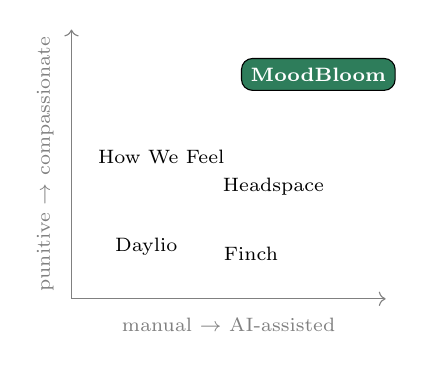
\begin{tikzpicture}[font=\scriptsize,scale=0.95]
    \draw[->,gray] (0,0) -- (4.2,0);
    \draw[->,gray] (0,0) -- (0,3.6);
    \node[rotate=90,gray] at (-0.35,1.8) {punitive $\to$ compassionate};
    \node[gray] at (2.1,-0.35) {manual $\to$ AI-assisted};
    \node[align=center] at (1.0,0.7) {Daylio};
    \node[align=center] at (1.2,1.9) {How We Feel};
    \node[align=center] at (2.4,0.6) {Finch};
    \node[align=center] at (2.7,1.5) {Headspace};
    \node[draw,rounded corners,fill=moodgreen,text=white,align=center] at (3.3,3.0) {\textbf{MoodBloom}};
  \end{tikzpicture}
  \end{column}
  \begin{column}{0.46\textwidth}
    \textbf{\color{moodgreen}\faCoins\ Business model}
    \begin{itemize}\small
      \item \textbf{Today:} cosmetic-only tokens (flower skins). Therapeutic features \emph{always} free.
      \item \textbf{Next:} optional cosmetic packs --- no premium currency, no paywalled insights.
      \item \textbf{Channel:} B2B2C via university counseling services, where our personas already live.
    \end{itemize}
  \end{column}
\end{columns}
\biz{The open quadrant is ours: AI-assisted \emph{and} compassionate. We monetize delight, never distress --- which is also why trust (and retention) is the moat.}
\note{Napat. Point to the empty top-right quadrant. Model: cosmetic-only, never paywall therapy; B2B2C via universities. Competitor placements are our analysis --- don't overclaim. speaker-script.md, Slide 5.}
\end{frame}

% ---- Slide 6 : Personas ----
\begin{frame}{Target Users \& Personas}
\begin{columns}[T,onlytextwidth]
  \begin{column}{0.48\textwidth}
    \textbf{\color{moodgreen}Lin --- everyday user (primary)}
    \begin{itemize}\small
      \item Third-year CS student, mild generalized anxiety.
      \item Goal: log a mood in under 30 seconds, daily.
      \item Pain: uninstalled three apps --- ``too naggy, too clinical.''
    \end{itemize}
  \end{column}
  \begin{column}{0.48\textwidth}
    \textbf{\color{moodorange}Som --- who safety exists for (secondary)}
    \begin{itemize}\small
      \item Going through a sustained low period.
      \item Goal: feel noticed without being alarmed or labeled.
      \item Pain: a wrong word at the wrong moment does real harm.
    \end{itemize}
  \end{column}
\end{columns}
\vfill
\centering{\color{moodgreendark}\textbf{Lin tests engagement. Som tests safety. Every feature answers to one of them.}}
\note{Napat. Humanize both; tagline is the product philosophy. Personas from docs/app-snapshot-for-personas.md. Hand demo to Jedsarit. speaker-script.md, Slide 6.}
\end{frame}

% ===================  SECTION 3 — LIVE DEMO  =========================

% ---- Slide 7 : Demo agenda ----
\begin{frame}{Live Demonstration --- Agenda}
  \begin{enumerate}
    \item \textbf{Cross-platform parity} --- log a mood on Android \emph{and} Web \hfill {\footnotesize($\sim$45s)}
    \item \textbf{Authentication} --- biometric / Privacy Lock / WebAuthn passkey (Web) \hfill {\footnotesize($\sim$30s)}
    \item \textbf{Offline-first} --- airplane mode $\to$ log $\to$ reconnect $\to$ Firestore sync \hfill {\footnotesize($\sim$30s)}
    \item \textbf{Accessibility} --- dynamic type to 200\%, dark-mode contrast \hfill {\footnotesize($\sim$30s)}
    \item \textbf{Intervention banner} --- canned (live trigger needs 14d of data) \hfill {\footnotesize($\sim$45s)}
  \end{enumerate}
  {\footnotesize\color{moodred}\faExclamationTriangle\ Every step has a pre-recorded fallback. If anything stalls, we cut to video and keep narrating.}
\note{Jedsarit. Five beats, $\sim$3 min. Promise backup videos up front. Tier-1 is canned by design. speaker-script.md, Slide 7.}
\end{frame}

% ---- Slide 8 : Cross-platform ----
\begin{frame}{Cross-Platform --- One Codebase, Two Targets}
\begin{columns}[c,onlytextwidth]
  \begin{column}{0.38\textwidth}\centering
    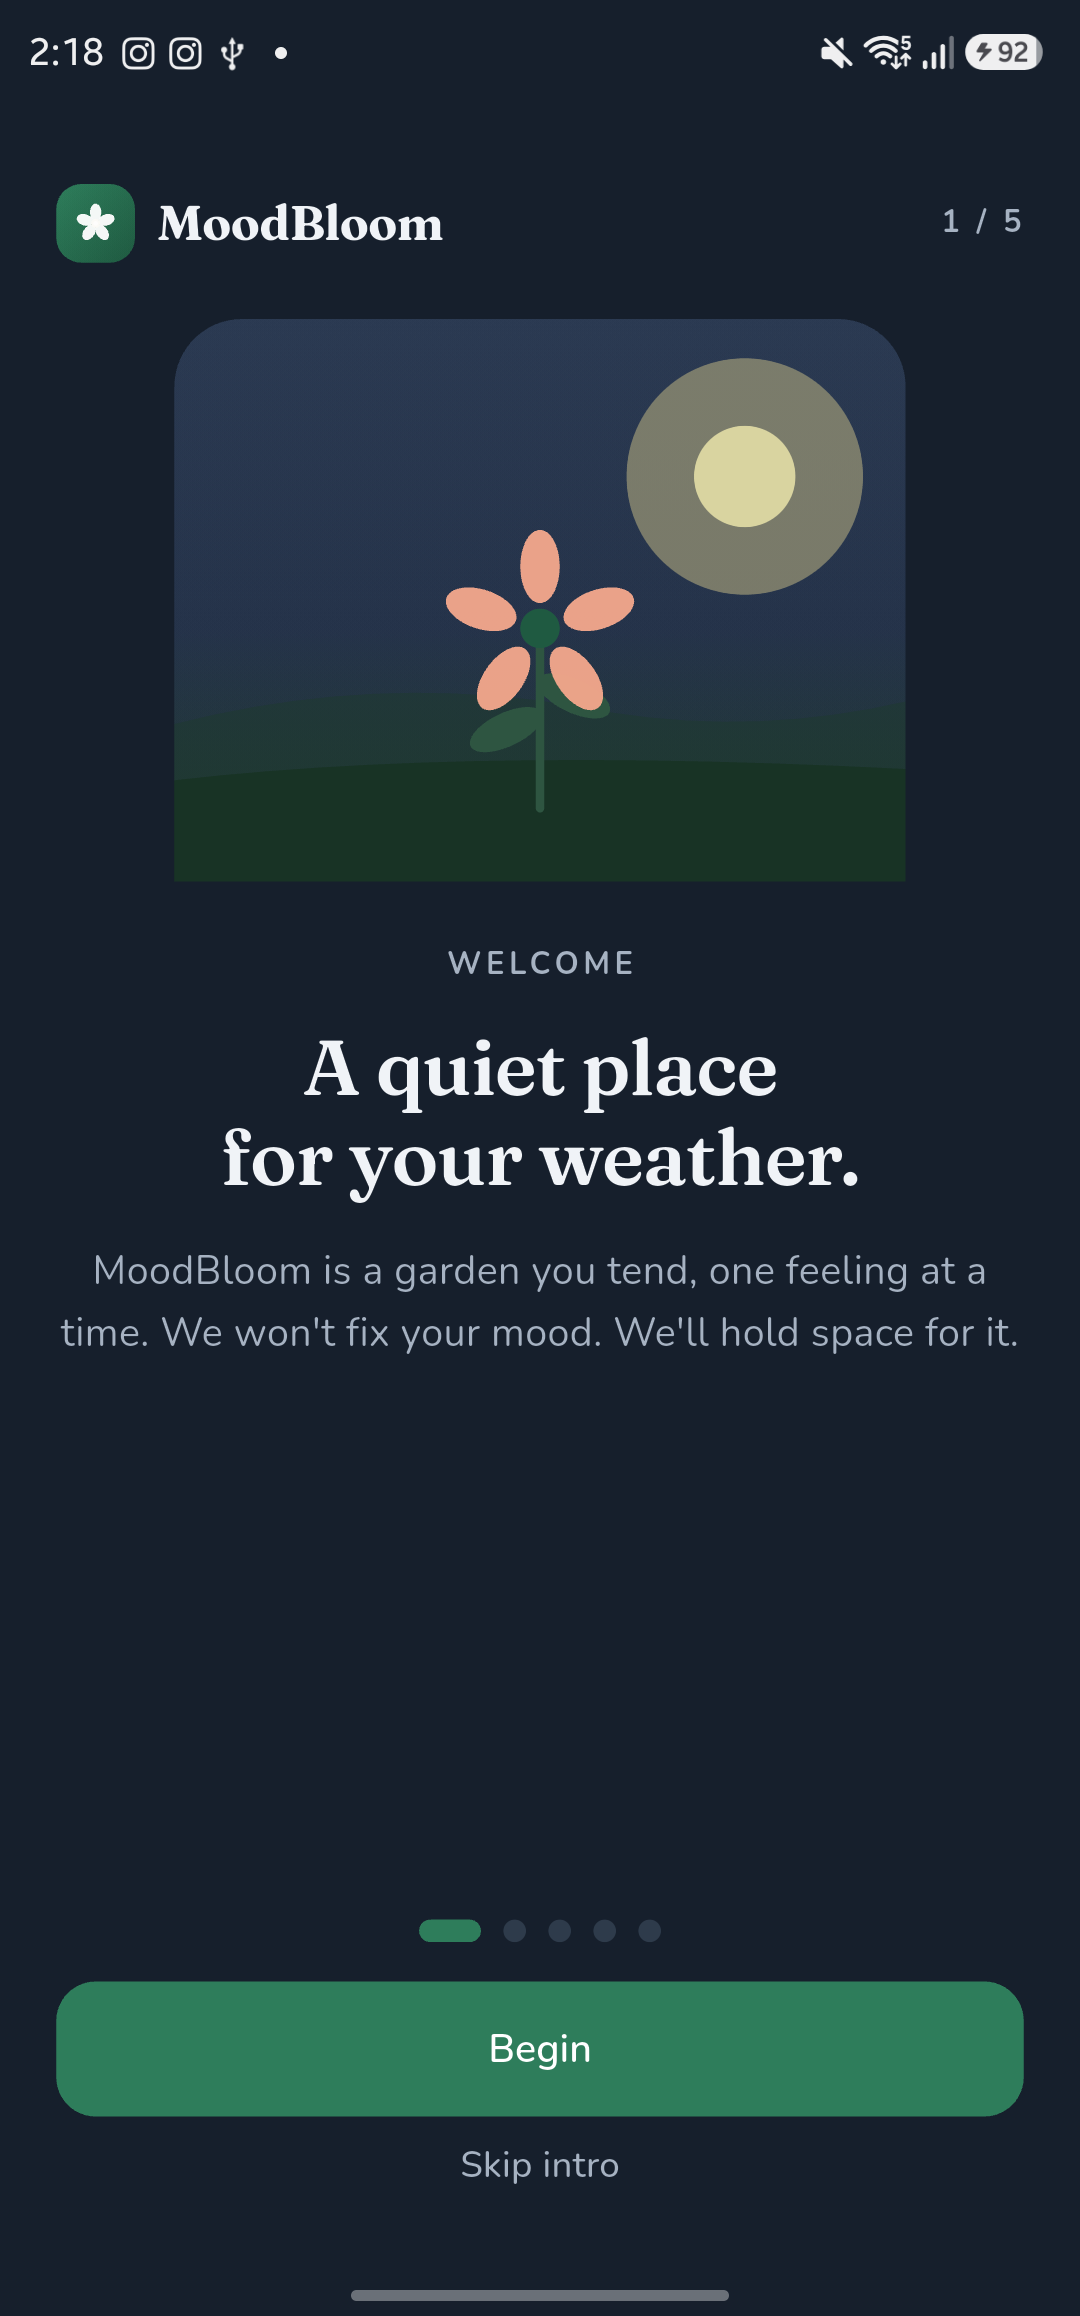
\includegraphics[height=0.60\textheight]{images/android-s23-onboarding-1-welcome.png}\\
    {\scriptsize \textbf{Android} --- Galaxy S23 Ultra, release APK}
  \end{column}
  \begin{column}{0.60\textwidth}\centering
    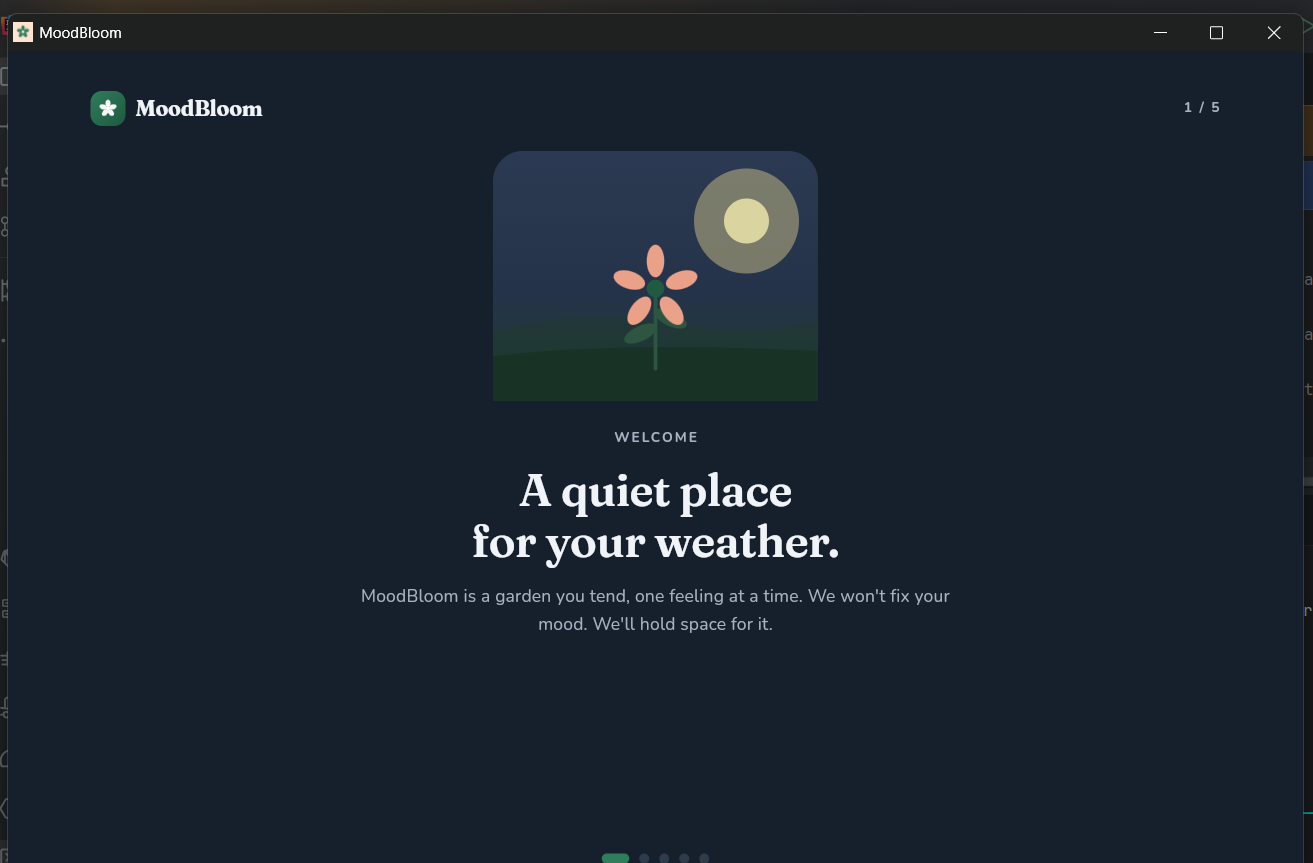
\includegraphics[width=\textwidth]{images/web-chrome-fullscreen.png}\\
    {\scriptsize \textbf{Web} --- Chrome 148, release build. Pixel-matched.}
  \end{column}
\end{columns}
\vspace{0.2em}
{\footnotesize\color{gray!70}One Dart codebase --- and the v1.6 patch redesign is \textbf{responsive} across phone, tablet, and desktop.}
\biz{One codebase $=$ one team, three form factors, two markets. No separate native builds to staff and maintain.}
\note{Jedsarit. [DO: log a mood live on the device, then on Web.] [FALLBACK: these two captures.] Same widget tree; v1.6 made it responsive phone/tablet/desktop. Honest note ready: web uses Firestore directly (Drift is native-only, ADR-0004). speaker-script.md, Slide 8.}
\end{frame}

% ---- Slide 9 : Enterprise features ----
\begin{frame}{Enterprise Features --- Under the Hood}
\begin{columns}[T,onlytextwidth]
  \begin{column}{0.49\textwidth}
    \textbf{\color{moodgreen}\faLock\ Authentication}\\
    {\footnotesize Firebase Auth + biometric (\texttt{local\_auth}) + 6-digit PIN (ADR-0013) + WebAuthn passkey, Web --- \textbf{shipped in the v1.6 patch} (ADR-0014).}\\[0.5em]
    \textbf{\color{moodgreen}\faLeaf\ Offline-first}\\
    {\footnotesize Drift (SQLite) write \emph{first}, then background mirror to Firestore --- the toast beats the network.}
  \end{column}
  \begin{column}{0.49\textwidth}
    \textbf{\color{moodgreen}\faCheckCircle\ Accessibility}\\
    {\footnotesize Dynamic type to 200\%, WCAG 2.2 AA contrast (light + dark), Semantics on every interactive widget.}\\[0.5em]
    \textbf{\color{moodgreen}\faChartLine\ Animated atmosphere}\\
    {\footnotesize Clouds, rain, butterflies on a seamless loop --- plants stay \emph{sheltered} even in Storm Season.}
  \end{column}
\end{columns}
\biz{Offline-first $=$ engagement survives the subway $=$ retention. A11y $=$ a larger addressable market and procurement-grade compliance.}
\note{Jedsarit drives; Teerin narrates a11y. [DO: airplane mode, log, reconnect, watch Firestore sync.] [FALLBACK: offline video.] [DO Teerin: type to 200\%, dark mode, TalkBack.] [FALLBACK: a11y video.] WebAuthn is now live (v1.6), not a foundation. speaker-script.md, Slide 9.}
\end{frame}

% ---- Slide 10 : Intervention banner ----
\begin{frame}{Intervention Banner --- Walkthrough (canned)}
  \centering
  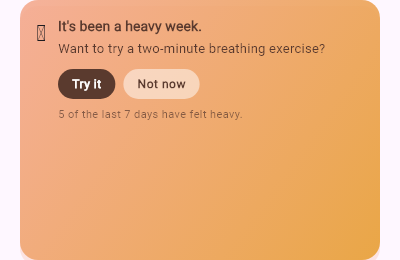
\includegraphics[height=0.44\textheight]{images/cheer_up_banner_5_of_7.png}\hfill
  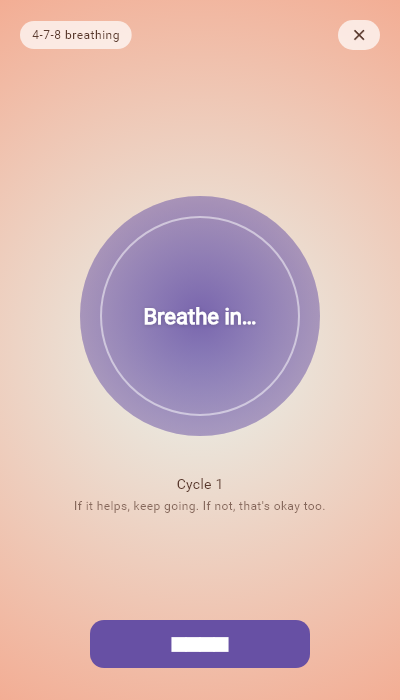
\includegraphics[height=0.44\textheight]{images/breathing_overlay_initial.png}
  \\[0.3em]
  {\footnotesize Pattern triggers $\to$ banner on Home $\to$ ``Open'' $\to$ 2-minute breathing sheet $\to$ cooldown timer in debug overlay.}\\
  {\footnotesize\color{moodred} Canned on purpose: a live Tier-1 needs 14 days of data, and the global cooldown blocks repeats --- the safety guard working.}
\note{Jedsarit. [DO: play the Tier-1 walkthrough video.] [FALLBACK: narrate these stills.] Explain why canned --- proves the guard works. Hand to Theerawat. speaker-script.md, Slide 10.}
\end{frame}

% ===============  SECTION 4 — MULTI-AGENT AI  ========================

% ---- Slide 11 : Four subagents ----
\begin{frame}{The Four Subagents}
\begin{columns}[T,onlytextwidth]
  \begin{column}{0.49\textwidth}
    \textbf{\color{moodgreen}architect.md}\\
    {\footnotesize Designs briefs, writes ADRs. \textit{Cannot:} write feature code or tests.}\\[0.5em]
    \textbf{\color{moodgreen}flutter-engineer.md}\\
    {\footnotesize Implements per brief. \textit{Cannot:} ``review your own work''; ``approve your own PR.''}
  \end{column}
  \begin{column}{0.49\textwidth}
    \textbf{\color{moodgreen}qa-engineer.md}\\
    {\footnotesize Widget/golden/integration tests, a11y, perf. \textit{Cannot:} ``lower coverage below 80\% on domain.''}\\[0.5em]
    \textbf{\color{moodgreen}security-reviewer.md}\\
    {\footnotesize Audits rules, CFs, secrets. \textit{Cannot:} ``READ-ONLY... not patches''; approve its own findings.}
  \end{column}
\end{columns}
\vfill
\centering{\color{moodgreendark}\textbf{Role-separation invariant: the implementer cannot approve their own work.}}
\note{Theerawat. Committee judges engineering maturity here. Hit the invariant. ``Cannot'' lines verbatim from .claude/agents/*.md. speaker-script.md, Slide 11.}
\end{frame}

% ---- Slide 12 : Plan Mode ----
\begin{frame}{Every Sprint Kickoff Starts in Plan Mode}
  \begin{quote}\itshape\color{moodgreendark}
  ``Enter Plan Mode. This is the highest-stakes sprint of the project --- Tier 3 messages must be byte-for-byte deterministic. Read carefully.''
  \end{quote}
  \hfill{\footnotesize --- \texttt{.claude/prompts/sprint-5-kickoff.md}}
  \vspace{0.6em}
  \begin{itemize}\small
    \item Orchestrator plans; humans approve; \emph{then} agents dispatch.
    \item Archived, not asserted: \texttt{docs/evidence/plan-mode/} holds six real sessions --- one reads \textit{``Approved via Ultraplan remote session\dots\ supersedes the prior local-orchestrator draft.''}
  \end{itemize}
\note{Theerawat. Read the quote aloud. Planning is a gate, and we can prove it ran --- six committed plan sessions. speaker-script.md, Slide 12.}
\end{frame}

% ---- Slide 13 : Human-in-the-loop ----
\begin{frame}{Human-in-the-Loop --- What We Caught That the AI Missed}
  \begin{enumerate}\small
    \item \textbf{S4 --- algorithm vs. reality.} An agent coded Mann-Kendall to a tolerance ($Z=-2.21\pm0.005$) an \emph{integer} statistic can't hit. Architect amended it to $\pm0.05$ in ADR-0011; tier semantics unchanged.
    \item \textbf{S5 --- privacy gap.} Day-2 audit found account-deletion drained Firestore but not Storage media at \texttt{users/\{uid\}/media/*}. Fixed in \texttt{c1ca5021}, re-verified.
    \item \textbf{S4 --- architectural drift.} A brief proposed merging two providers ``for simplicity.'' Orchestrator rejected the coupling; kept separate --- later proven right.
  \end{enumerate}
  \biz{Governed AI, not unmanaged AI --- the difference an enterprise buyer diligences.}
\note{Theerawat. Be specific and honest --- committee WILL probe. Three real, documented catches; none shipped. speaker-script.md, Slide 13.}
\end{frame}

% ---- Slide 14 : Handoff briefs (+ Orchestration ROI folded in) ----
\begin{frame}{The Handoff Brief is the Unit of Work}
\begin{columns}[T,onlytextwidth]
  \begin{column}{0.46\textwidth}
    \textbf{HB-007 --- structure:}
    \begin{itemize}\footnotesize
      \item Goal \textperiodcentered\ Inputs
      \item Files to create \textperiodcentered\ Files to extend
      \item Dispatcher state machine
      \item Cooldown guard rules
      \item Acceptance \textperiodcentered\ Open questions \textperiodcentered\ Non-goals
    \end{itemize}
    {\footnotesize Three shipped this way: HB-007 dispatcher, HB-008 quote filter, HB-009 Insights.}
  \end{column}
  \begin{column}{0.50\textwidth}
    \textbf{\color{moodgreen}\faBalanceScale\ What the model bought us}
    \begin{itemize}\footnotesize
      \item 5 sprints \textperiodcentered\ 5 people $\to$ 157 commits, 1{,}139 tests, 14 ADRs.
      \item \textbf{Velocity:} role-scoped agents + briefs $=$ parallel delivery.
      \item \textbf{Governance:} ADRs (audit trail) + enforced hooks + role-separation.
      \item \textbf{Cost \& risk:} fewer people, traceable decisions, reproducible builds.
    \end{itemize}
  \end{column}
\end{columns}
\biz{A repeatable \emph{delivery model}, not a one-off demo. Sharpen the brief and the implementation follows --- a vague brief drifts, even from the best model.}
\note{Theerawat. The brief --- not the agent --- is the unit of work. Right column folds in the orchestration ROI: velocity, governance, cost --- the modern-engineering-management story the committee wants. Hand to Kraiwich. speaker-script.md, Slide 14.}
\end{frame}

% ===============  SECTION 5 — ARCHITECTURE & DATA  ===================

% ---- Slide 15 : Clean Architecture ----
\begin{frame}{Enterprise Architecture --- Clean, Three-Layer}
\centering
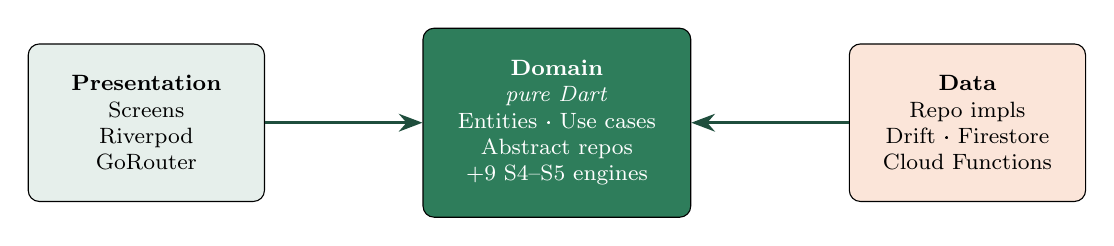
\begin{tikzpicture}[font=\footnotesize]
  \node[draw,rounded corners,fill=moodgreen!12,minimum width=3.0cm,minimum height=2.0cm,align=center] (pres) {\textbf{Presentation}\\Screens\\Riverpod\\GoRouter};
  \node[draw,rounded corners,fill=moodgreen,text=white,minimum width=3.4cm,minimum height=2.4cm,align=center,right=2.0cm of pres] (dom) {\textbf{Domain}\\\textit{pure Dart}\\Entities \textperiodcentered\ Use cases\\Abstract repos\\+9 S4--S5 engines};
  \node[draw,rounded corners,fill=moodorange!15,minimum width=3.0cm,minimum height=2.0cm,align=center,right=2.0cm of dom] (data) {\textbf{Data}\\Repo impls\\Drift \textperiodcentered\ Firestore\\Cloud Functions};
  \draw[-{Stealth[length=3mm]},very thick,moodgreendark] (pres) -- (dom);
  \draw[-{Stealth[length=3mm]},very thick,moodgreendark] (data) -- (dom);
\end{tikzpicture}
\vspace{0.3em}
\begin{itemize}\footnotesize
  \item Dependencies point \textbf{inward}. Domain depends on nothing but pure Dart.
  \item \textbf{Zero} \texttt{package:flutter}/\texttt{firebase\_*} imports in \texttt{domain/} --- enforced by a commit hook (\texttt{.claude/hooks/settings.json}), not a guideline.
\end{itemize}
\note{Kraiwich. Arrows inward to a pure-Dart domain. Purity is ENFORCED by a hook --- the whole ecosystem unit-tests without a Flutter binding. Those nine engines are next. speaker-script.md, Slide 15.}
\end{frame}

% ---- Slide 16 : Pattern Engine — Five Algorithms ----
\begin{frame}{The Pattern Engine --- Five Algorithms, Five Failure Modes}
{\footnotesize Every entry updates $S_t = v\cdot(i/5)\in[-1,+1]$, then $H_t = 0.15\,S_t + 0.85\,H_{t-1}$, then runs five pure-Dart detectors:}
\vspace{0.2em}
\begin{center}\scriptsize
\begin{tabular}{@{}lll@{}}
\toprule
\textbf{Algorithm} & \textbf{Failure mode it catches} & \textbf{Threshold $\to$ Tier} \\
\midrule
Mann-Kendall (14d) & gradual worsening & $Z_{\text{trend}} < -1.96 \to$ T1 \\
Sliding 5-of-7 & sustained lows & $\geq 5$ neg.\ days / 7 $\to$ T2 \\
3-Consecutive & acute crisis & $S \leq -0.6$ for 3 days $\to$ T3 \\
Z-score (vs 30d) & one-off alarming day & $z_{\text{day}} < -2.5 \to$ T3 \\
CUSUM & sudden sustained shift & $C_t > 4\sigma_{30} \to$ T3 \\
\bottomrule
\end{tabular}
\end{center}
\vspace{0.2em}
\begin{columns}[T,onlytextwidth]
  \begin{column}{0.54\textwidth}
    {\footnotesize\textbf{Mann-Kendall:} $S=\sum_{i<j}\operatorname{sign}(x_j-x_i)$,\ \ $Z=\dfrac{S\mp 1}{\sqrt{V}}$,\ \ $V=\dfrac{n(n{-}1)(2n{+}5)}{18}$. Two-tailed $1.96$ over one-tailed $1.645$: fewer false alarms.}
  \end{column}
  \begin{column}{0.42\textwidth}
    {\footnotesize $z_{\text{day}}$ (sudden crash vs 30-day baseline) is \emph{not} $Z_{\text{trend}}$ (14-day gradual). Same letter, different math.\\ {\scriptsize Mann 1945 \textperiodcentered\ Page 1954 \textperiodcentered\ Nahum-Shani 2018.}}
  \end{column}
\end{columns}
\biz{Five lenses, no blind spot --- and it runs \emph{on-device} in pure Dart: zero inference cost, instant, unit-testable without a network.}
\note{Kraiwich. The depth the commentators will probe. Walk the table: each algorithm = a distinct failure mode. Mann-Kendall is the 14-day trend; z-day is the single-day crash --- same letter, different math. All pure Dart, on-device, no server inference cost. Full math for the other four is in Appendix A4. speaker-script.md, Slide 16.}
\end{frame}

% ---- Slide 17 : State & Navigation ----
\begin{frame}{State \& Navigation}
\begin{columns}[T,onlytextwidth]
  \begin{column}{0.49\textwidth}
    \textbf{\color{moodgreen}State --- Riverpod (@riverpod)}
    \begin{itemize}\footnotesize
      \item Family providers for per-user state.
      \item \texttt{AsyncValue} unifies loading/error/data.
      \item e.g. \texttt{gardenStateStreamProvider}, \texttt{interventionStateProvider}.
    \end{itemize}
  \end{column}
  \begin{column}{0.49\textwidth}
    \textbf{\color{moodgreen}Navigation --- GoRouter}
    \begin{itemize}\footnotesize
      \item \texttt{StatefulShellRoute.indexedStack} --- 5 tabs (\texttt{router.dart:272}).
      \item Auth (\texttt{:194}), onboarding (\texttt{:190}), privacy-lock (\texttt{:199--222}) guards.
      \item Lock redirect preserves intent: \texttt{?returnTo=\dots}
    \end{itemize}
  \end{column}
\end{columns}
\note{Kraiwich. Riverpod codegen + AsyncValue; GoRouter indexed-stack with three stacked guards; privacy guard preserves the return route. Real line numbers. speaker-script.md, Slide 17.}
\end{frame}

% ---- Slide 18 : Firestore ----
\begin{frame}[fragile]{Cloud Data Strategy --- Firestore}
\begin{columns}[T,onlytextwidth]
  \begin{column}{0.52\textwidth}
{\scriptsize Per-user tree + the moods update rule:}
\begin{lstlisting}[style=rulestyle]
users/{uid}/moods/{moodId}
users/{uid}/weeklyGardens/{weekId}
users/{uid}/patterns/{date}
allow update: if isOwner(uid)      // RBAC
 && resource.data.createdAt ==
    request.resource.data.createdAt // immutable
 && diff(resource.data).affectedKeys()
    .hasOnly(['mood','intensity',
      'text','mediaRefs','updatedAt']);
\end{lstlisting}
  \end{column}
  \begin{column}{0.46\textwidth}
    \textbf{\color{moodgreen}Design}
    \begin{itemize}\footnotesize
      \item \textbf{RBAC:} \texttt{isOwner} --- you touch only your own subtree.
      \item \textbf{Field allowlist:} \texttt{diff().affectedKeys().hasOnly} blocks smuggled fields.
      \item \textbf{Denormalized:} \texttt{weeklyGardens} stores a rich snapshot (\texttt{entries[]}, \texttt{healthHistory[]}, \texttt{summary}) --- reads stay single-document.
      \item \textbf{Indexing:} per-user, single-collection, time-ordered $\Rightarrow$ Firestore's \emph{automatic} indexes suffice; no composite-index burden.
    \end{itemize}
  \end{column}
\end{columns}
\biz{Per-user isolation $+$ field-level rules $=$ breach blast-radius of one account. That's the line an enterprise security review starts at.}
\note{Kraiwich. Read the rule guarantees: RBAC, immutable createdAt, field allowlist. Denormalized weekly snapshot keeps reads single-doc; access patterns need no composite indexes. Full rule is Appendix A2. speaker-script.md, Slide 18.}
\end{frame}

% ===============  SECTION 6 — RELIABILITY & QUALITY GATES  ==========

% ---- Slide 19 : Four Quality Gates ----
\begin{frame}{Enterprise Readiness --- Four Quality Gates}
\begin{columns}[T,onlytextwidth]
  \begin{column}{0.49\textwidth}
    \textbf{\color{moodgreen}Correctness}\\
    {\footnotesize \textbf{1,045} Flutter + \textbf{94} Cloud Function tests pass ($=$ \textbf{1,139}). Domain coverage 94.6\%--100\% (gate: 80\%).}\\[0.4em]
    \textbf{\color{moodgreen}Security}\\
    {\footnotesize Zero open HIGH/CRITICAL; zero plaintext secrets (secret-scan hook); per-user Firestore isolation; rules emulator-tested.}
  \end{column}
  \begin{column}{0.49\textwidth}
    \textbf{\color{moodgreen}Accessibility}\\
    {\footnotesize 53 a11y tests + WCAG 2.2 AA contrast sweep (light + dark) --- Tier-3 affordances 7.2:1, body 14:1. \emph{1 dark pair tracked for a token fix.}}\\[0.4em]
    \textbf{\color{moodgreen}Performance}\\
    {\footnotesize Static review: 0 HIGH + device cold-start runbook. \emph{1 tracked MEDIUM: image caching (\texttt{cached\_network\_image}).}}
  \end{column}
\end{columns}
\biz{All four gates are the diligence checklist of an enterprise buyer --- and all four are \emph{documented}, with the two open optimizations named, not hidden.}
{\footnotesize\color{gray!70} Counts: \texttt{docs/evidence/platform-execution/} (2026-05-31). a11y/perf: \texttt{docs/test-reports/}. Full breakdown: Appendix A8.}
\note{Teerin. Numbers not adjectives. a11y and perf are documented strengths now: 53 a11y tests + contrast sweeps; static perf review 0 HIGH. Name the two open optimizations honestly. speaker-script.md, Slide 19.}
\end{frame}

% ---- Slide 20 : Tier 3 determinism ----
\begin{frame}[fragile]{Tier 3 Determinism --- The Most Important Test We Wrote}
\begin{columns}[T,onlytextwidth]
  \begin{column}{0.49\textwidth}
{\footnotesize TC-40 --- Tier 3 never reaches Gemini:}
\begin{lstlisting}[style=dartstyle]
await dispatcher.dispatch(
    tier: Tier.three, ...);
expect(ai.calls, isEmpty,
  reason: 'ADR-0012: Tier 3 '
  'must never reach Gemini.');
expect(dispatch.body,
  contains('1323'));
\end{lstlisting}
  \end{column}
  \begin{column}{0.49\textwidth}
{\footnotesize TC-41 --- 55 adversarial inputs, 100\% rejected:}
\begin{lstlisting}[style=dartstyle]
// 25 forbidden + 15 over-length
// + 10 off-script + 5 almost-OK
for (final s in adversarial) {
  filter.gate(s,
    tier: AiAllowedTier.one);
}
expect(passThroughs, 0);
\end{lstlisting}
  \end{column}
\end{columns}
\vspace{0.1em}
\centering{\footnotesize\color{moodgreendark}\textbf{Type-level fence \texttt{enum AiAllowedTier \{ one, two \}} + runtime branch + unit test + integration test.}}
\biz{The single largest legal/trust risk in a wellness product --- a harmful auto-generated message to a vulnerable user --- engineered out at the type level.}
\note{Teerin. Left TC-40: ai.calls empty --- Gemini never invoked. Right TC-41: 55 adversarial strings, zero pass-throughs. The fence is type-level: Tier.three won't compile into the AI path. Full enum source: Appendix A3. speaker-script.md, Slide 20.}
\end{frame}

% ---- Slide 21 : Observability ----
\begin{frame}{Observability --- Crashlytics + Structured Logging}
\begin{columns}[T,onlytextwidth]
  \begin{column}{0.49\textwidth}
    \textbf{\color{moodred}What we deliberately do NOT log}
    \begin{itemize}\footnotesize
      \item Mood text content (PII)
      \item Email + uid pairs
      \item Gemini request/response bodies
    \end{itemize}
  \end{column}
  \begin{column}{0.49\textwidth}
    \textbf{\color{moodgreen}Feature flags (Remote Config)}
    \begin{itemize}\footnotesize
      \item \texttt{ai\_pattern\_analysis\_enabled}
      \item \texttt{intervention\_dispatch\_enabled}
      \item \texttt{gemini\_detection\_enabled}
    \end{itemize}
  \end{column}
\end{columns}
\vfill
{\footnotesize\color{gray!70} Crashlytics + a structured logger in \texttt{packages/core}; \texttt{print()} is blocked outside tests by a write hook.}
\note{Teerin. Observability is also a privacy posture --- never log mood text, email+uid, or Gemini bodies. Three flags set up the rollback story. speaker-script.md, Slide 21.}
\end{frame}

% ---- Slide 22 : Rollback ----
\begin{frame}{Feature-Flag Rollback Plan}
\renewcommand{\arraystretch}{1.3}
\begin{tabularx}{\textwidth}{>{\raggedright\arraybackslash}p{0.28\textwidth} >{\raggedright\arraybackslash}p{0.30\textwidth} >{\raggedright\arraybackslash}X}
\toprule
\textbf{Scenario} & \textbf{Flag to flip} & \textbf{Behavior after} \\
\midrule
Gemini misbehaves on quotes & \texttt{ai\_pattern\_analysis\_enabled = false} & Tier 1/2 fall back to curated phrases; Tier 3 unaffected \\
Dispatcher critical bug & \texttt{intervention\_dispatch\_enabled = false} & No notifications; detection continues in Insights \\
Bad AI mood suggestions & \texttt{gemini\_detection\_enabled = false} & AI pill disappears; manual selection works \\
\bottomrule
\end{tabularx}
\vfill
{\footnotesize\color{moodred}\textbf{Tier 3 cannot be rolled back via flag --- it never uses Gemini. The only Tier 3 ``rollback'' is a client update. By design.}}
\note{Teerin. Three levers, each a single flip with a safe degradation. Red line: Tier 3 has nothing to roll back. Hand to Theerawat. speaker-script.md, Slide 22.}
\end{frame}

% ===============  SECTION 7 — CONCLUSION  ============================

% ---- Slide 23 : Summary of value ----
\begin{frame}{Summary of Value}
  \begin{enumerate}
    \item \textbf{Business} --- a retention-first wedge into a $\sim$US\$20B market; monetize delight, never distress.
    \item \textbf{Therapeutic safety} --- deterministic Tier 3, a disclaimer in five places, mood-agnostic gamification.
    \item \textbf{Enterprise readiness} --- 1{,}139 tests, type-level safety fences, RBAC isolation, observable, rollback-capable.
  \end{enumerate}
  \vfill
  \centering{\Large\color{moodgreendark}\itshape ``A garden you can audit --- and a business you can defend.''}
\note{Theerawat. Three claims --- business, safety, enterprise readiness. Tagline lands the whole pitch. speaker-script.md, Slide 23.}
\end{frame}

% ---- Slide 24 : Lessons + CTA ----
\begin{frame}{Lessons Learned \& Next Steps}
  \begin{itemize}
    \item \textbf{On AI orchestration:} the handoff brief is the unit of work --- sharpen the brief, the implementation follows.
    \item \textbf{On safety:} when the user is most vulnerable, the code must be most \emph{boring}. Tier 3 has no AI by design.
    \item \textbf{Shipped in v1.6} (the Sprint 5 patch wave)\textbf{:} responsive phone/tablet/desktop redesign + WebAuthn passkeys live. \textbf{Next:} image-cache optimization, the final dark-contrast token, a published runtime perf trace.
  \end{itemize}
  \vfill
  \centering
  {\color{moodgreendark}\textbf{We're open for the committee's technical audit and questions.}}\\[0.5em]
  {\footnotesize\ttfamily repo: github.com/<org>/csc234-project-2025 \textperiodcentered\ CLAUDE.md \textperiodcentered\ v1.6 \textperiodcentered\ 0e55021a}
\note{Theerawat. Two lessons + what v1.6 shipped + the honest next items, then open Q\&A. Have repo, CLAUDE.md, ADR-0012, HB-007 tabs ready. [CLAUDE\_CODE\_FILL: confirm public repo URL/org.] speaker-script.md, Slide 24.}
\end{frame}

% =====================================================================
%  APPENDIX — Technical backup for Q&A. NOT presented in the main run.
%  Beamer's \appendix resets numbering so the main deck stays "24 of 24".
%  Each slide maps to a likely committee drill — jump to it on demand.
%  See qa-prep.md (question → appendix slide) and speaker-script.md index.
% =====================================================================
\appendix

\begin{frame}[plain]
  \centering\vfill
  {\Large\bfseries\color{moodgreendark} Appendix --- Technical Backup}\\[0.4em]
  {\footnotesize\color{gray!70} Not presented. Held for the committee's technical audit.\\
  A1 EWMA \textperiodcentered\ A2 Firestore rule \textperiodcentered\ A3 Type fence \textperiodcentered\ A4 Pattern math\\
  A5 Cooldown \textperiodcentered\ A6 Account deletion \textperiodcentered\ A7 Disclaimer \textperiodcentered\ A8 Test pyramid}
  \vfill
  \note{Divider. Do not present. Jump here only when a commentator drills in. The map: which slide answers which question is in qa-prep.md and speaker-script.md's appendix index.}
\end{frame}

% ---- A1 : EWMA worked example + tiers ----
\begin{frame}{A1 \textperiodcentered\ Garden Health EWMA --- worked example}
{\footnotesize $H_t = \alpha S_t + (1-\alpha)H_{t-1}$,\quad $\alpha = 0.15$,\quad $H_0 = 0$ (resets weekly).}
\vspace{0.3em}
\begin{columns}[T,onlytextwidth]
  \begin{column}{0.52\textwidth}
    {\footnotesize\textbf{Why $\alpha=0.15$:} $\alpha \approx 2/(N{+}1)$ gives a $\sim$13-day window --- aligned to PHQ-9's 2-week period. A single day can move $H$ by at most $0.15$, so the garden \emph{cannot} drop more than one tier in a day.}
    \vspace{0.5em}
    {\footnotesize\textbf{Three-day walk:}}
    \begin{itemize}\footnotesize
      \item $S=+0.6 \Rightarrow H_1 = 0.15(0.6)+0.85(0) = +0.09$
      \item $S=-0.8 \Rightarrow H_2 = 0.15(-0.8)+0.85(0.09) = -0.04$
      \item $S=+0.4 \Rightarrow H_3 = 0.15(0.4)+0.85(-0.04) = +0.03$
    \end{itemize}
    {\footnotesize A brutal $-0.8$ day only nudges $H$ from $+0.09$ to $-0.04$ --- still ``Resting,'' never collapse.}
  \end{column}
  \begin{column}{0.44\textwidth}
  {\scriptsize
  \begin{tabular}{@{}ll@{}}
  \toprule
  $H_t$ & State \\
  \midrule
  $\geq +0.4$ & Flourishing \\
  $[+0.1,+0.4)$ & Thriving \\
  $[-0.1,+0.1)$ & Resting \\
  $[-0.4,-0.1)$ & Weathering \\
  $< -0.4$ & Storm Season \\
  \bottomrule
  \end{tabular}}
  \\[0.4em]{\scriptsize All five tiers are alive. Citations: Smit et al.\ (2022); Kroenke et al.\ (2001).}
  \end{column}
\end{columns}
\note{Backs Q13 (mood-score quality) + ``why 0.15?''. The bound is the whole point: max $\pm0.15$/day means no single day collapses the garden. Numbers are verbatim from spec §2.3.}
\end{frame}

% ---- A2 : Firestore moods rule, full verbatim ----
\begin{frame}[fragile]{A2 \textperiodcentered\ Firestore --- the real \texttt{moods} rule (verbatim)}
\begin{lstlisting}[style=rulestyle,basicstyle=\ttfamily\tiny]
function isOwner(uid) { return request.auth != null && request.auth.uid == uid; }

// same-day edit window; createdAt immutable; field-level allowlist
allow update: if isOwner(uid)
  && request.time.year()  == resource.data.createdAt.year()
  && request.time.month() == resource.data.createdAt.month()
  && request.time.day()   == resource.data.createdAt.day()
  && request.resource.data.createdAt == resource.data.createdAt
  && request.resource.data.updatedAt is timestamp
  && request.resource.data.updatedAt == request.time
  && request.resource.data.diff(resource.data).affectedKeys()
       .hasOnly(['mood','intensity','text','mediaRefs','updatedAt'])
  && request.resource.data.intensity is int
  && request.resource.data.intensity >= 1 && request.resource.data.intensity <= 5
  && request.resource.data.text.size() <= 500
  && request.resource.data.mood in ['happy','calm','okay','sad','angry','anxious'];
\end{lstlisting}
{\footnotesize Plus a one-way field guard on \texttt{users/\{uid\}}: \texttt{insightsDisclaimerAcked} can go \texttt{false$\to$true} but never back --- the client cannot un-acknowledge the medical disclaimer.}
\note{Backs Q1 (diff() pattern). This is firestore.rules:55--69 verbatim. Walk the four guard classes: same-day window, createdAt immutability, type+range validation, field allowlist. The one-way ack guard is a second field-level RBAC example.}
\end{frame}

% ---- A3 : Type-level fence, full source ----
\begin{frame}[fragile]{A3 \textperiodcentered\ The Tier-3 type fence (verbatim source)}
\begin{lstlisting}[style=dartstyle]
enum AiAllowedTier {
  one,
  two;

  // Lifts Tier to AiAllowedTier. Throws on Tier.three by construction.
  static AiAllowedTier fromTier(Tier t) => switch (t) {
    Tier.one => AiAllowedTier.one,
    Tier.two => AiAllowedTier.two,
    Tier.three => throw StateError(
      'AiAllowedTier.fromTier called with Tier.three - '
      'invariant violated. Tier 3 must never reach the AI path.'),
  };
}
\end{lstlisting}
{\footnotesize \texttt{AIQuoteRepository.requestSuggestion} accepts \texttt{AiAllowedTier}, \emph{not} \texttt{Tier}. Two fences: (1) the dispatcher's \texttt{if (tier == Tier.three)} arm returns first; (2) even if a future refactor deletes that arm, \texttt{fromTier} throws --- and TC-40 catches it before production.}
\note{Backs Q2 (walk the enum). The enum has only one and two --- Tier.three is unrepresentable in the AI path. The StateError is belt-and-suspenders for a future refactor. ai\_allowed\_tier.dart verbatim.}
\end{frame}

% ---- A4 : Pattern engine — full math ----
\begin{frame}{A4 \textperiodcentered\ Pattern Engine --- the other four detectors}
\begin{columns}[T,onlytextwidth]
  \begin{column}{0.5\textwidth}
    {\footnotesize\textbf{Sliding 5-of-7} (Tier 2)}\\
    {\footnotesize $\text{neg\_days}=\lvert\{S_t<0 \text{ in last 7}\}\rvert \geq 5$. Mirrors PHQ-9 ``more than half the days.''}
    \vspace{0.5em}
    {\footnotesize\textbf{3-Consecutive} (Tier 3)}\\
    {\footnotesize $S_{t-2}\leq-0.6 \,\wedge\, S_{t-1}\leq-0.6 \,\wedge\, S_t\leq-0.6$.}
    \vspace{0.5em}
    {\footnotesize\textbf{Z-score / single-day} (Tier 3)}\\
    {\footnotesize $z_{\text{day}} = \dfrac{S_t - \mu_{30}}{\sigma_{30}}$,\quad $z_{\text{day}} < -2.5$.}
  \end{column}
  \begin{column}{0.46\textwidth}
    {\footnotesize\textbf{CUSUM change-point} (Tier 3)}\\
    {\footnotesize $C_t = \max\!\big(0,\; C_{t-1} + (\mu_{30}-k) - S_t\big)$\\[0.3em]
    $k = 0.5\,\sigma_{30}$ (slack),\quad $h = 4\,\sigma_{30}$ (threshold)\\[0.3em]
    Fire when $C_t > h$.}
    \vspace{0.6em}
    {\scriptsize $z_{\text{day}}$ (sudden crash vs 30-day baseline) is \emph{not} $Z_{\text{trend}}$ (14-day Mann-Kendall). Same letter, different statistic. Citations: Mann (1945), Page (1954), Nahum-Shani (2018).}
  \end{column}
\end{columns}
\note{Backs the algorithm drill (companion to main Slide 16, which typeset Mann-Kendall). Each detector is a distinct failure mode; thresholds verbatim from spec §2.4. Emphasize z\_day vs Z\_trend again if asked.}
\end{frame}

% ---- A5 : Cooldown state machine ----
\begin{frame}{A5 \textperiodcentered\ Intervention cooldown --- persistence \& guard}
\begin{itemize}\footnotesize
  \item \textbf{Global across tiers} (HB-007 OQ-B): one shared anchor blocks \emph{any} tier from re-firing. A dismissed Tier-1 can't surface a jarring Tier-3 the next day.
  \item \textbf{Rules:} max 1 notification / 24h; 48h between alerts; opt-out (``I'm okay'') on every tier.
  \item \textbf{Persistence:} anchors (\texttt{lastTriggeredAt}, \texttt{firstTriggeredAt}) in Firestore at \texttt{users/\{uid\}/interventionState/current}, mirrored to local \texttt{SharedPreferences} for offline reads.
  \item \textbf{Fail-closed:} if \emph{both} the Firestore read and the local mirror fail, the guard returns \texttt{Blocked} --- never risk a double-notify.
\end{itemize}
\vfill
{\footnotesize\color{gray!70} ADR-0008 \textperiodcentered\ \texttt{cooldown\_guard.dart:35,38,53--56} \textperiodcentered\ TC-31/TC-32.}
\note{Backs Q15 (cooldown persistence/restart). Survives restart because the anchor is in Firestore + SharedPrefs. Global, not per-tier, was a human override of an agent's per-tier proposal. Fail-closed is the safety default.}
\end{frame}

% ---- A6 : Account deletion cascade ----
\begin{frame}{A6 \textperiodcentered\ Account deletion --- end-to-end cascade}
\begin{itemize}\footnotesize
  \item Single callable Cloud Function \texttt{wipeUserData} (\texttt{asia-southeast1}); reauth required before the call.
  \item Admin-SDK cascade: \texttt{db.recursiveDelete(users/\{uid\})} $\to$ \texttt{bucket.deleteFiles(users/\{uid\}/media/)} $\to$ \texttt{admin.auth().deleteUser(uid)}.
  \item Idempotent --- ``not found'' is treated as success; partial-failure path still returns \texttt{ok: true}.
  \item \textbf{The human catch (R-H01):} the first version drained Firestore but \emph{not} Storage media. Day-2 security audit caught it; fixed in \texttt{c1ca5021}; re-verified in the final posture report.
\end{itemize}
\vfill
{\footnotesize\color{gray!70} ADR-0009 \textperiodcentered\ \texttt{functions/src/wipeUserData.ts} \textperiodcentered\ supports right-to-erasure (formal DPA review before a GDPR-certified claim).}
\note{Backs Q11 (deletion / GDPR). Walk the three cascade steps. The R-H01 storage gap is one of our three documented human catches --- lean on it as proof of governance.}
\end{frame}

% ---- A7 : Disclaimer — 5 placements + verbatim copy ----
\begin{frame}{A7 \textperiodcentered\ Medical disclaimer --- five placements}
{\footnotesize\itshape ``MoodBloom is not a medical device. It cannot diagnose conditions like bipolar disorder, depression, or anxiety. The patterns and insights it shows are observational only. If you're concerned about your mental health, please consult a qualified professional.''}
\vspace{0.4em}
\begin{enumerate}\footnotesize
  \item \textbf{Onboarding} slide (first launch).
  \item \textbf{Insights} screen --- non-dismissible ack dialog on first view; persisted to \texttt{users/\{uid\}.insightsDisclaimerAcked} (and one-way at the rules layer, see A2).
  \item \textbf{Every Tier 1/2/3 notification} footer (short form).
  \item \textbf{Settings $\to$ About} --- always available.
  \item \textbf{Crisis (Tier 3)} resources screen + Hotline 1323.
\end{enumerate}
\vfill
{\footnotesize\color{gray!70} Copy is byte-for-byte locked in \texttt{disclaimer\_copy.dart}; \texttt{disclaimer\_copy\_test.dart} asserts each constant.}
\note{Backs therapeutic-safety / HIPAA drills (Q12). Full copy is verbatim from disclaimer\_copy.dart. The ack is enforced two ways: persisted flag + one-way Firestore rule. Five surfaces = defense in depth on the safety message.}
\end{frame}

% ---- A8 : Test pyramid + coverage ----
\begin{frame}{A8 \textperiodcentered\ Test pyramid \& coverage}
\begin{columns}[T,onlytextwidth]
  \begin{column}{0.52\textwidth}
    \begin{itemize}\footnotesize
      \item \textbf{1,045} Flutter tests (unit + widget + golden) --- \texttt{flutter test --exclude-tags=golden,shader} logs \texttt{+1045: All tests passed!}
      \item \textbf{94} Cloud Function tests (7 Jest suites) --- \texttt{94 passed, 94 total}.
      \item \textbf{= 1,139} total, on committed 2026-05-31 logs.
      \item Domain coverage \textbf{94.6\%--100\%} per feature (gate: 80\%).
      \item \textbf{53} dedicated a11y tests + WCAG contrast sweeps (light + dark).
    \end{itemize}
  \end{column}
  \begin{column}{0.44\textwidth}
    {\footnotesize\textbf{Honest caveats (documented):}}
    \begin{itemize}\footnotesize
      \item On-device integration run: 1/4 passed --- a device-timing/pump-budget issue, not an app failure (the app boots + renders; screenshots prove it).
      \item Web unit suite doesn't compile under Chrome \emph{by design} --- Drift is native-only (ADR-0004); logic is covered by the 1,045 host-VM tests both platforms share.
    \end{itemize}
  \end{column}
\end{columns}
\vfill
{\footnotesize\color{gray!70} \texttt{docs/evidence/platform-execution/} (README + logs).}
\note{Backs Q3 (coverage) + Q26 (1018 vs 1045). Be ready with the two honest caveats --- they read as maturity, not weakness. The v1.5 tag was 1018; the +27 are v1.6/FCM tests in the same run.}
\end{frame}

\end{document}
